\documentclass[aspectratio=169]{beamer}
\usepackage{will_handley_beamer}
\usepackage{title_page}
\usepackage{slashed}

% Commands
% --------
% - \arxiv{arxiv number}
% - \cols{width}{lh column}{rh column}
% -  \begin{fig(left|right)}[fractional width (e.g 0.6) ]{name of image}
%        content of other column
%    \end{fig(left|right)}

% Talk details
% ------------
\title{Next-generation astrophysical inference\\across the interdisciplinary frontier}
\date{29\textsuperscript{th} April 2024}

\begin{document}

\begin{frame}
    \titlepage
\end{frame}

\begin{frame}
    \frametitle{Beginning the golden age of astronomy data}
    \begin{columns}
        \column{0.45\textwidth}
        \begin{itemize}
            \item Over our research lifetimes we will see next-generation data rates across the electromagnetic spectrum \& beyond:
                \begin{description}
                    \item[Radio] SKA \textit{et al}
                    \item[Micro] SO/CMB-S4
                    \item[IR] JWST, Roman (WFIRST)
                    \item[Optical] Euclid, DESI, Rubin (LSST), EELT
                    \item[X-ray] Athena
                    \item[Gamma-ray] e-ASTROGAM
                    \item[Gravitational] LIGO/Virgo/Kagra + LISA
                    \item[Particle] CTA, IceCube, KM3NeT
                \end{description}
        \end{itemize}
        \column{0.55\textwidth}

        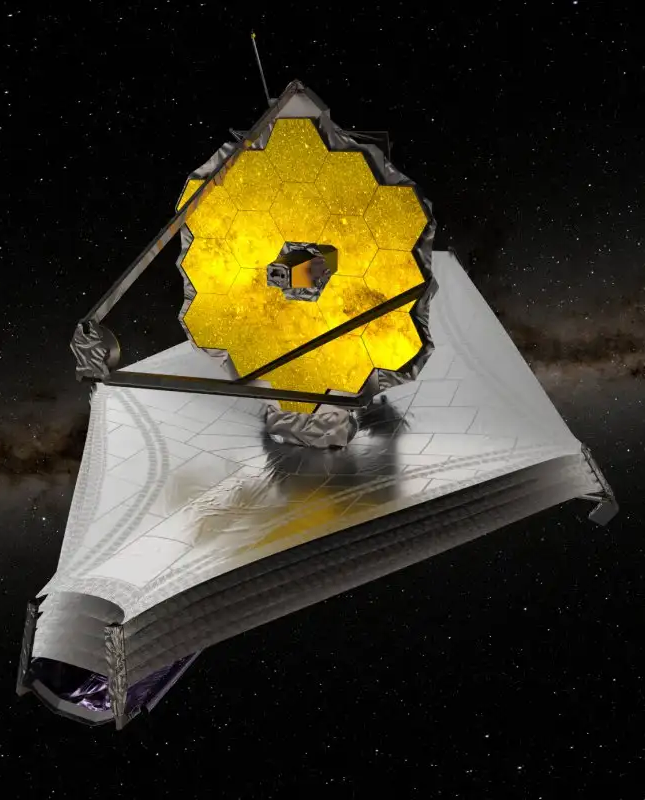
\includegraphics[height=0.145\textwidth]{figures/telescopes/jwst.png}%
        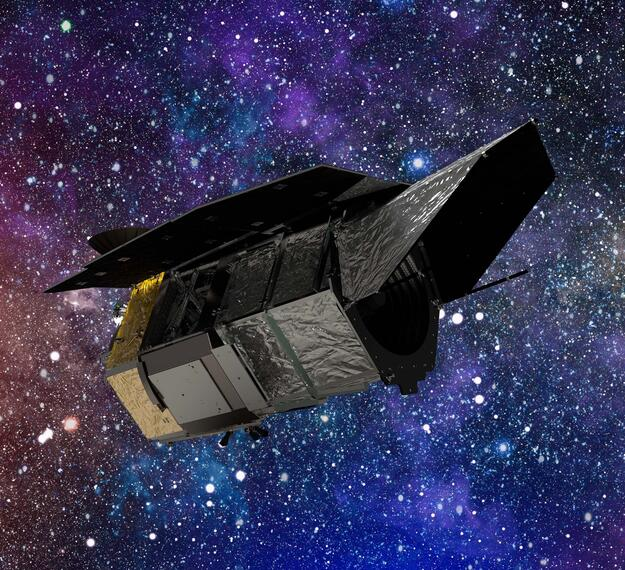
\includegraphics[height=0.145\textwidth]{figures/telescopes/roman.jpg}%
        \includegraphics[height=0.145\textwidth]{figures/telescopes/euclid.jpeg}%
        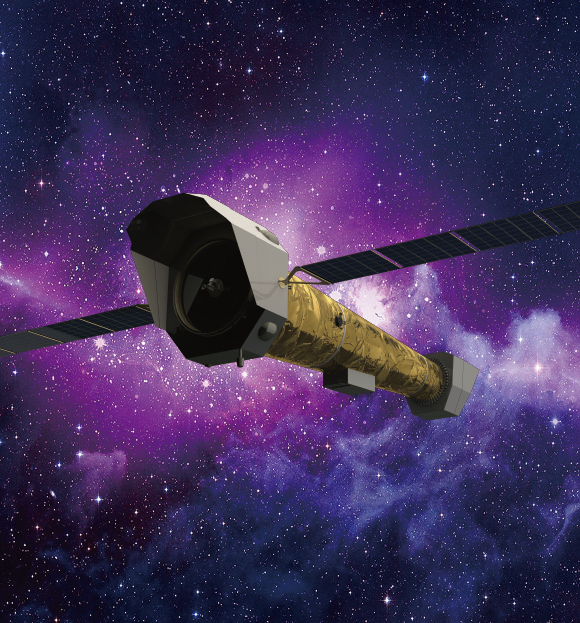
\includegraphics[height=0.145\textwidth]{figures/telescopes/athena.jpg}%
        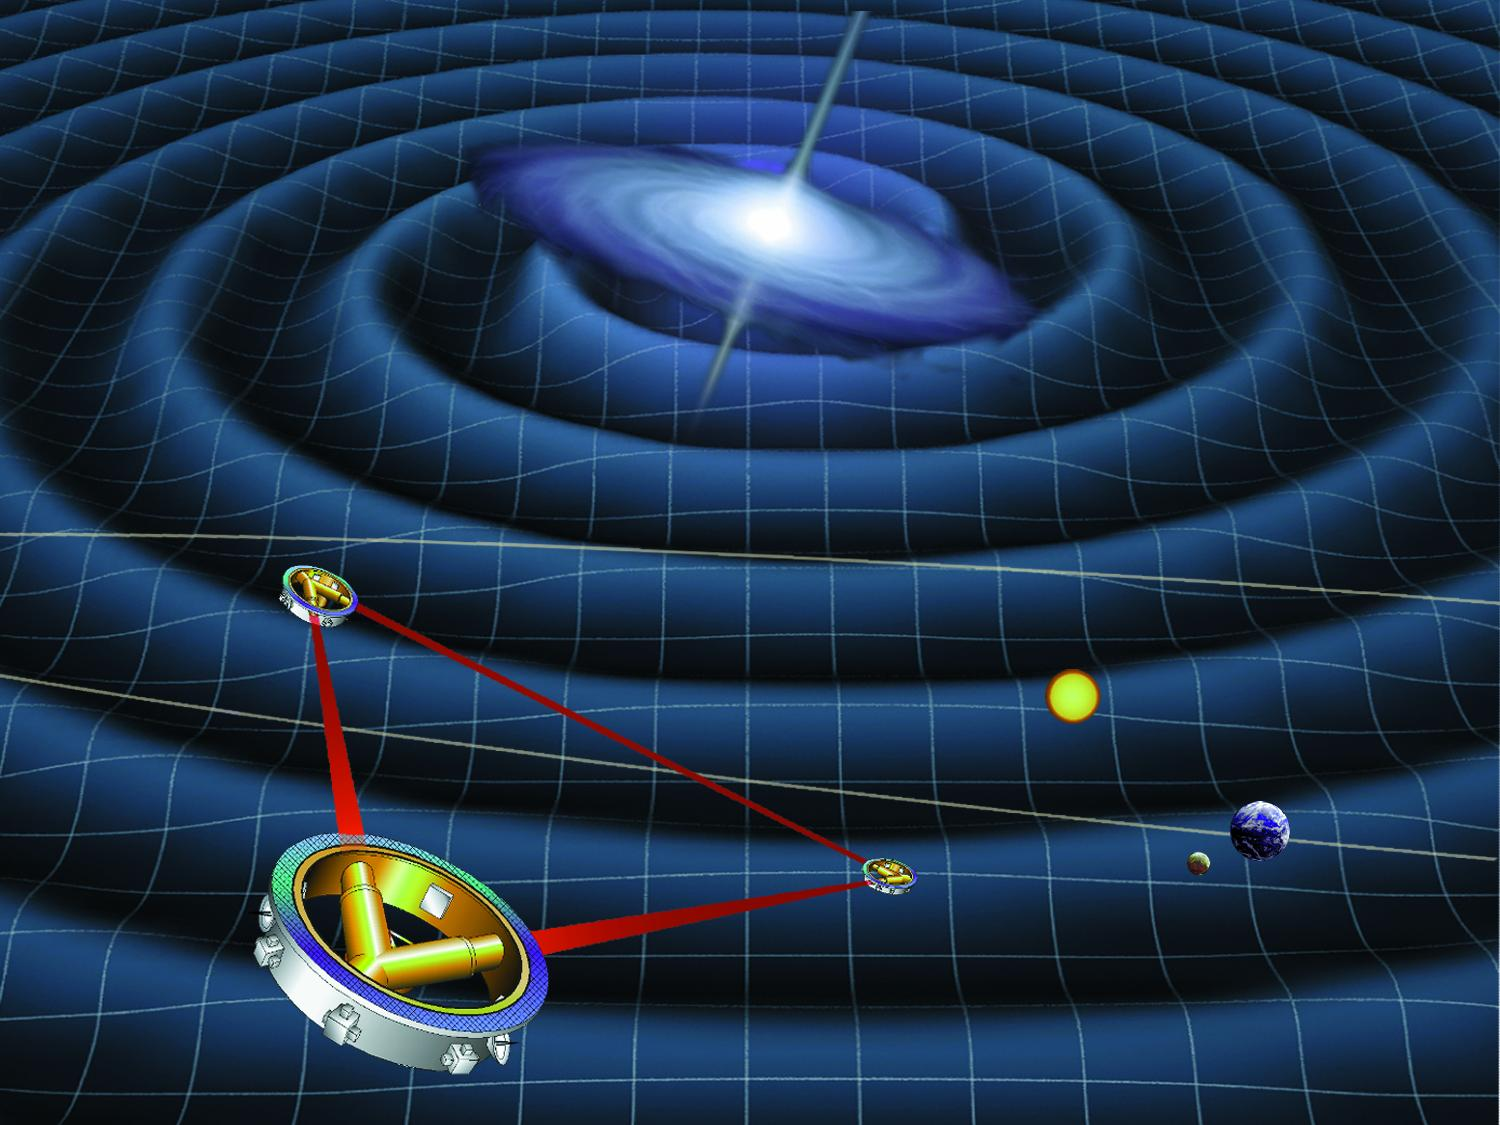
\includegraphics[height=0.145\textwidth]{figures/telescopes/lisa.jpg}%
        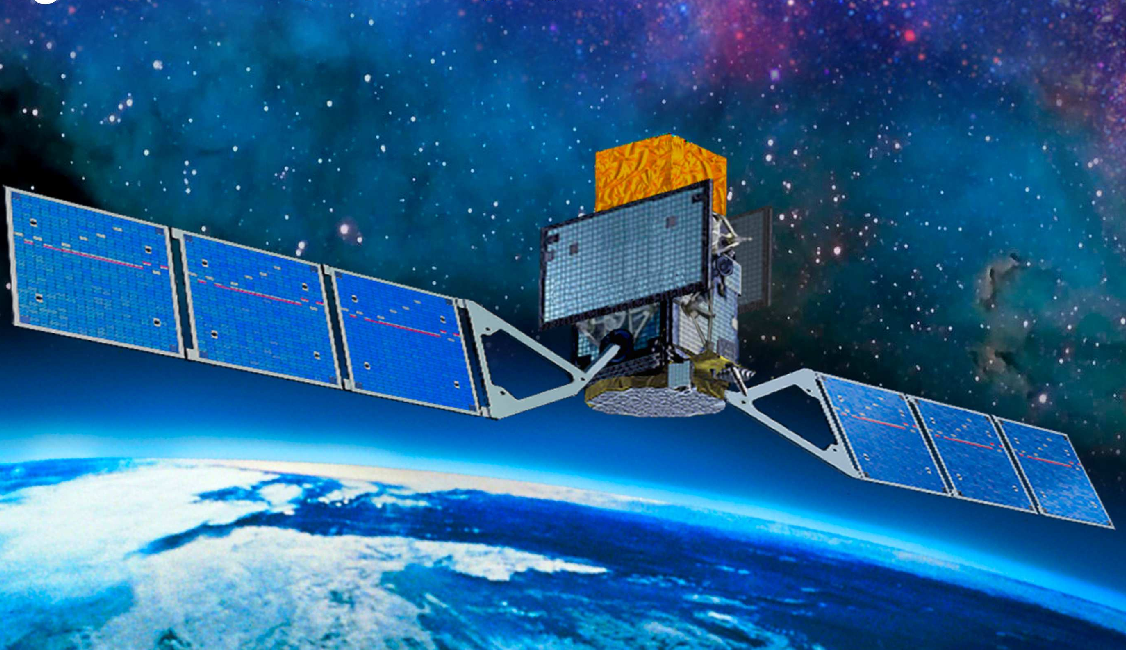
\includegraphics[height=0.145\textwidth]{figures/telescopes/e-ASTROGAM.pdf}%
        \vspace{-1pt}

        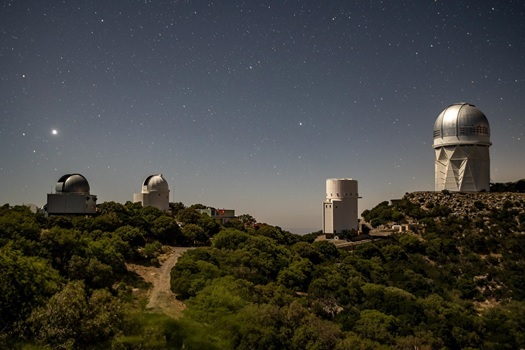
\includegraphics[height=0.15183\textwidth]{figures/telescopes/desi.jpg}%
        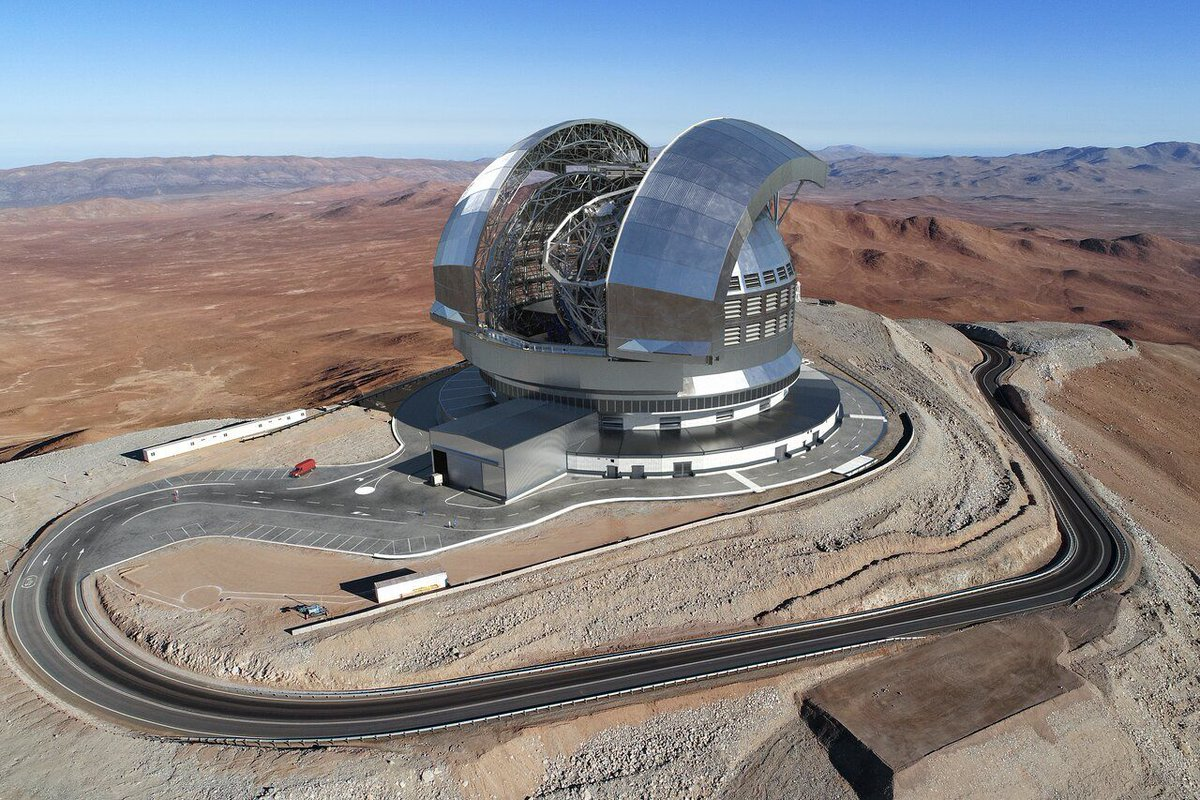
\includegraphics[height=0.15183\textwidth]{figures/telescopes/eelt.jpg}%
        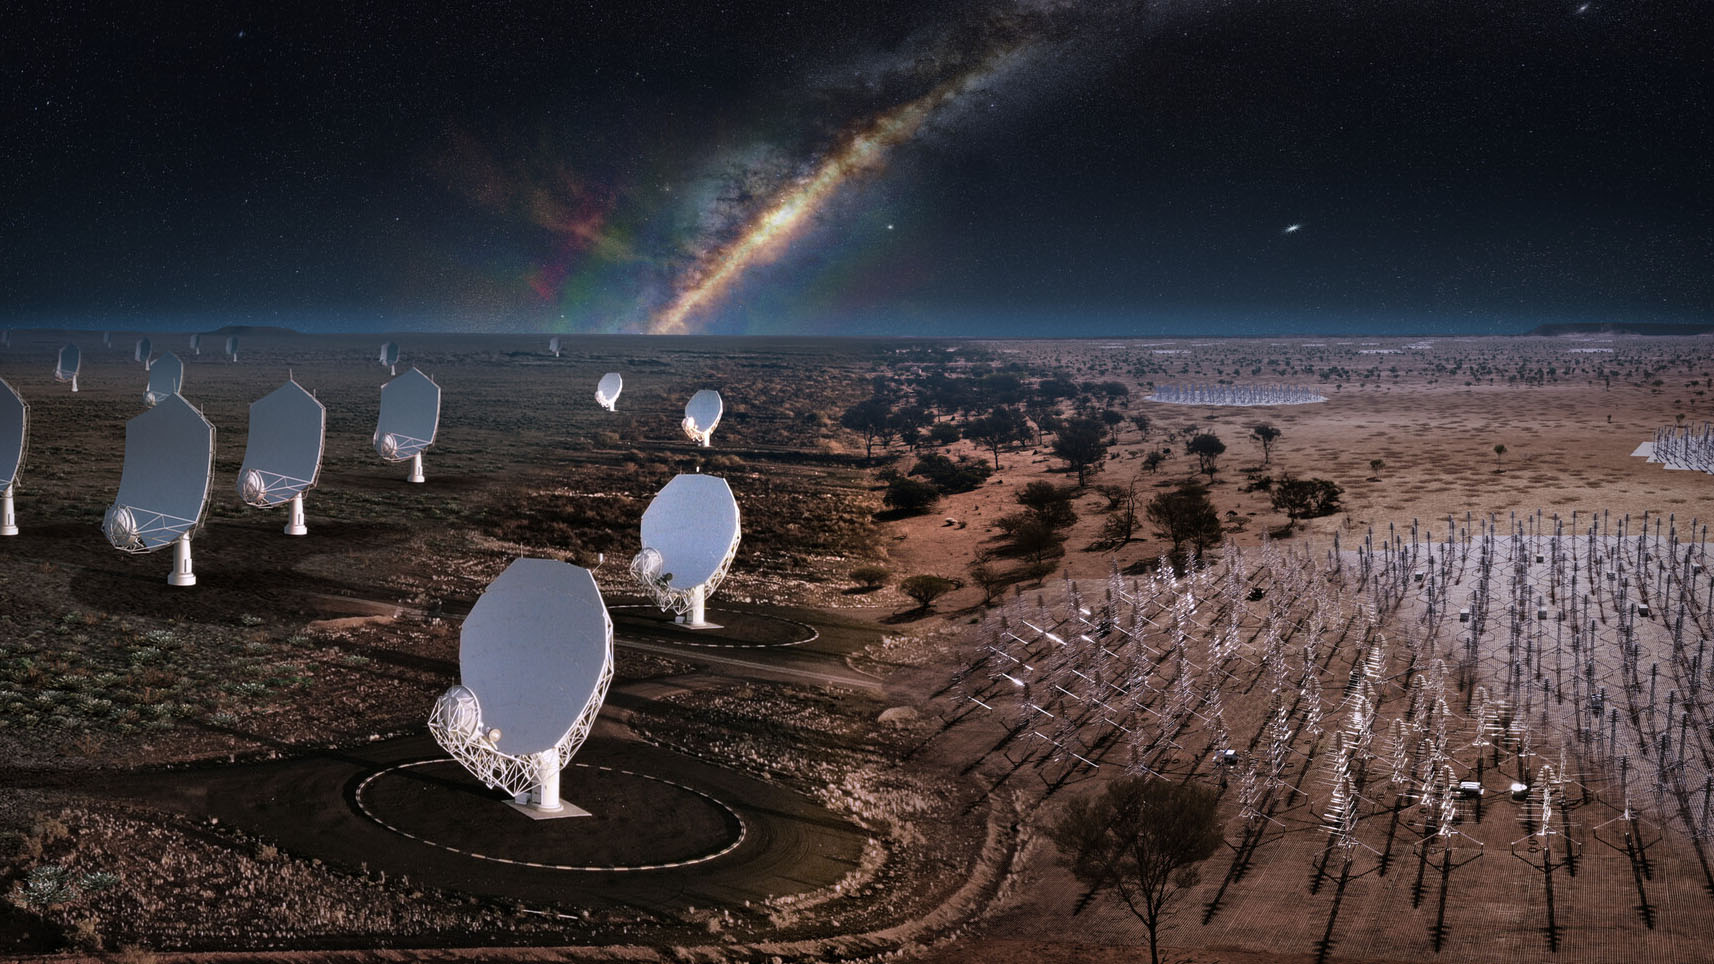
\includegraphics[height=0.15183\textwidth]{figures/telescopes/ska.jpg}%
        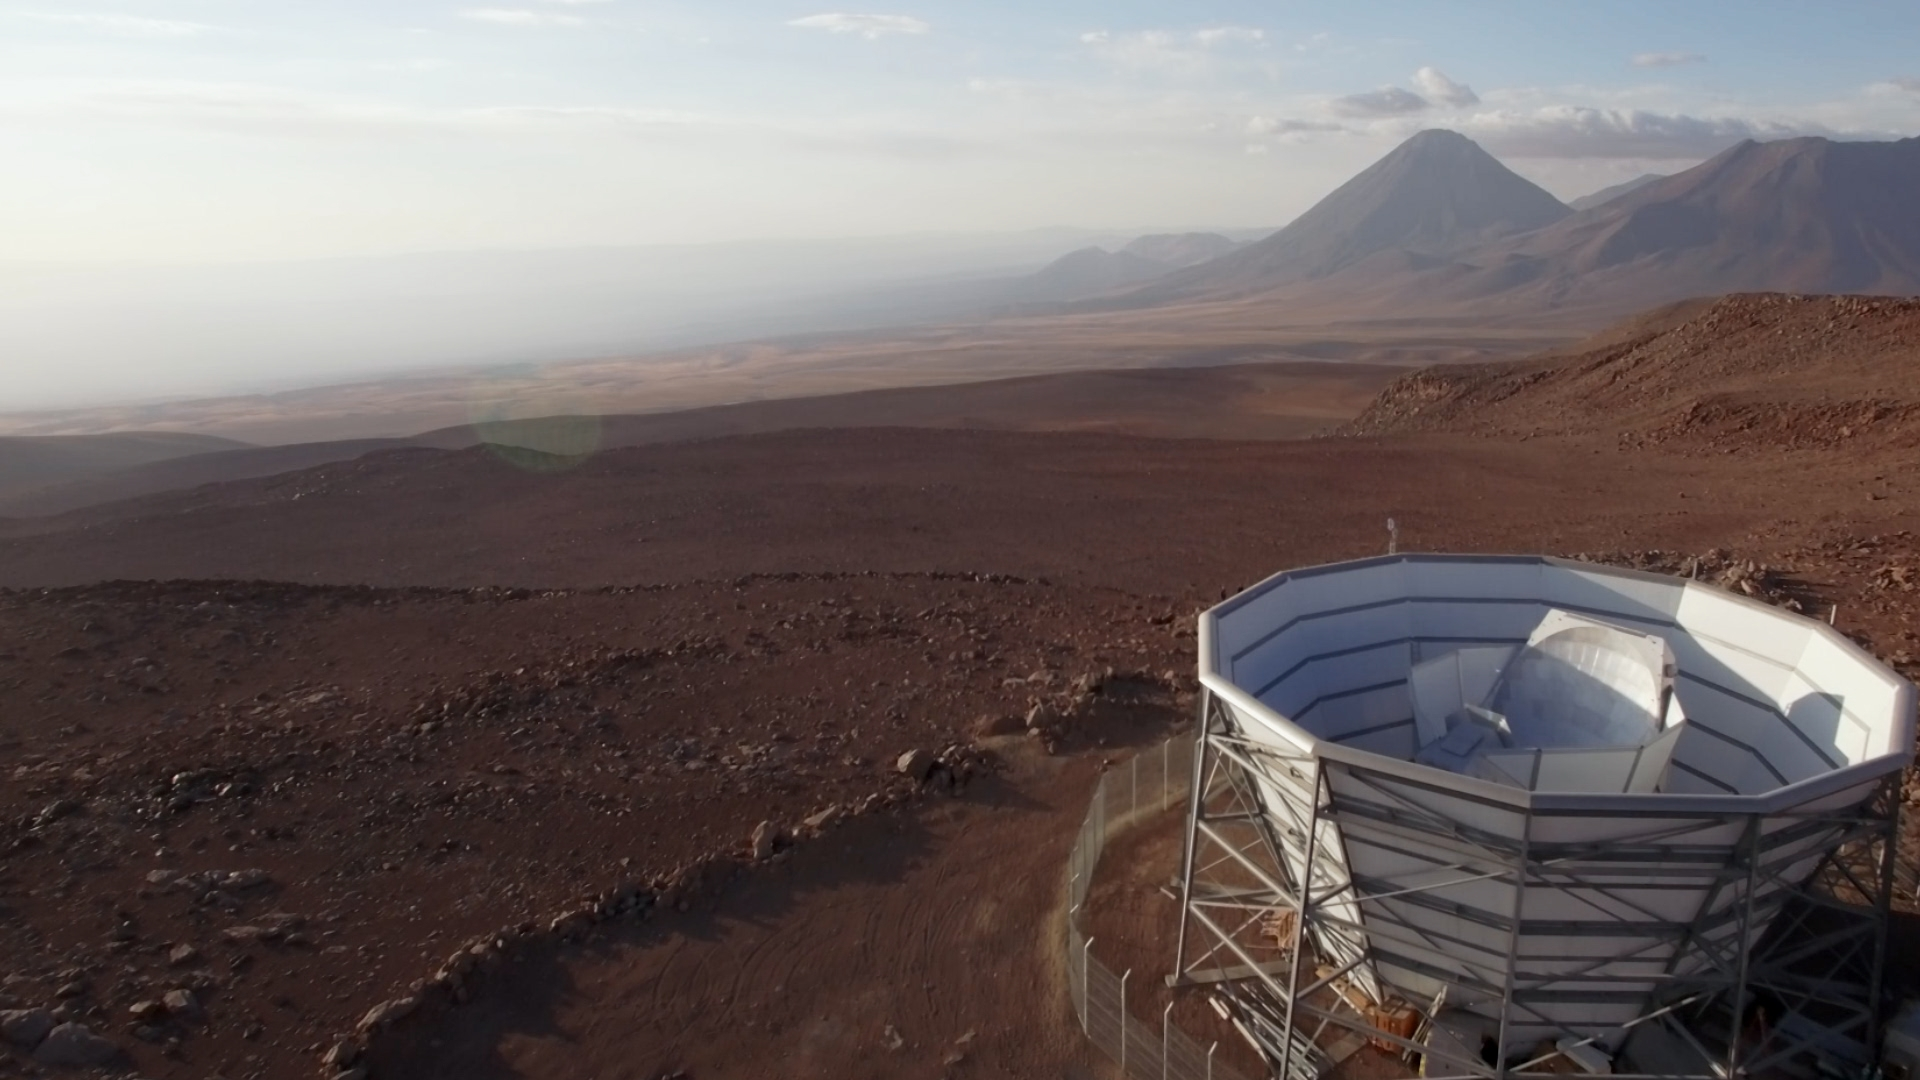
\includegraphics[height=0.15183\textwidth]{figures/telescopes/SO.jpg}%
        \vspace{-1pt}

        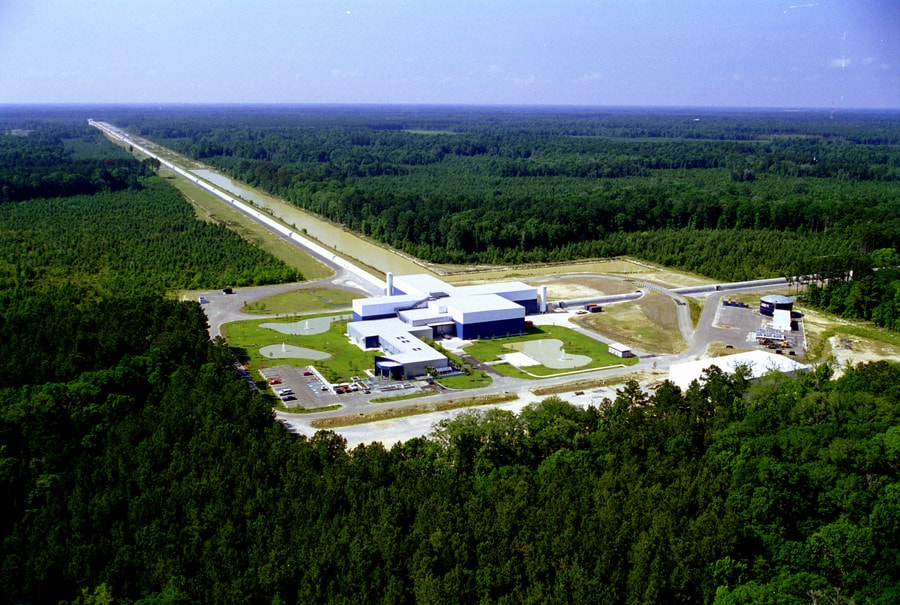
\includegraphics[height=0.18428\textwidth]{figures/telescopes/ligo.jpg}%
        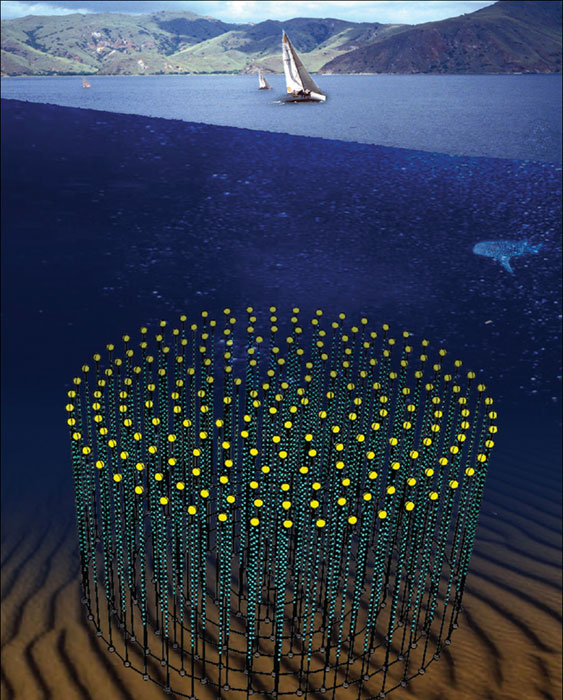
\includegraphics[height=0.18428\textwidth]{figures/telescopes/km3n.jpg}%
        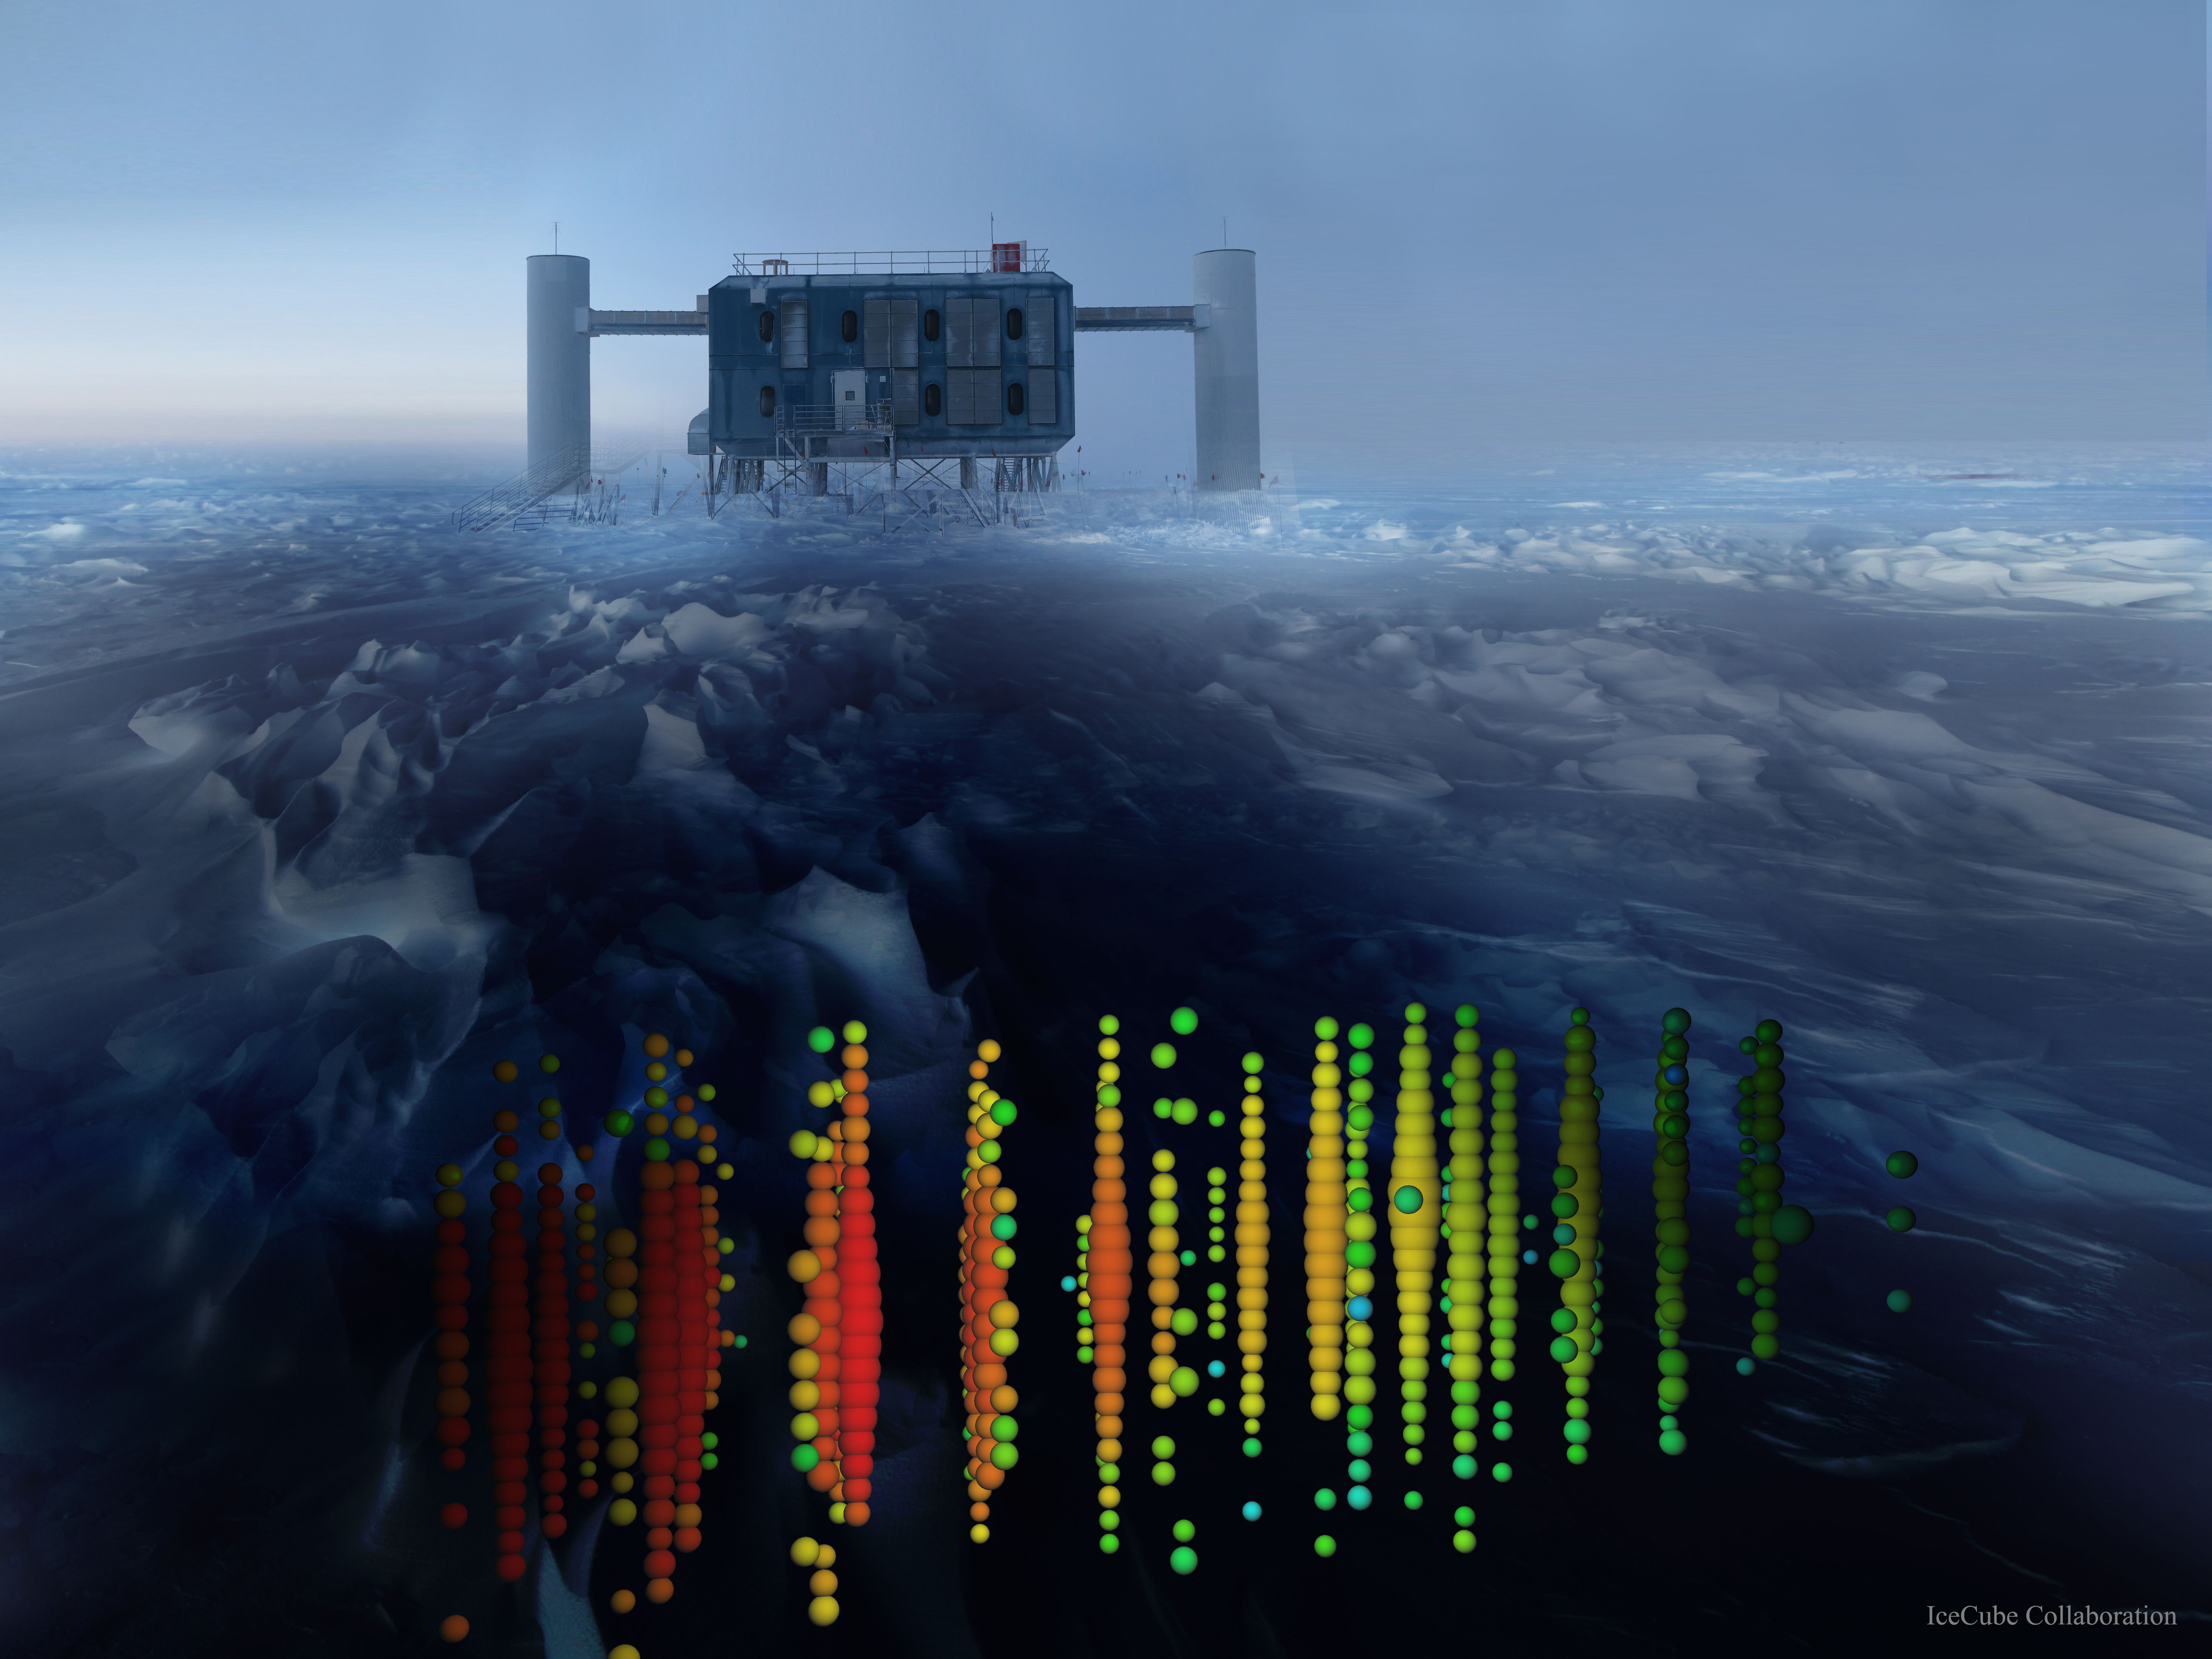
\includegraphics[height=0.18428\textwidth]{figures/telescopes/icecube.jpg}%
        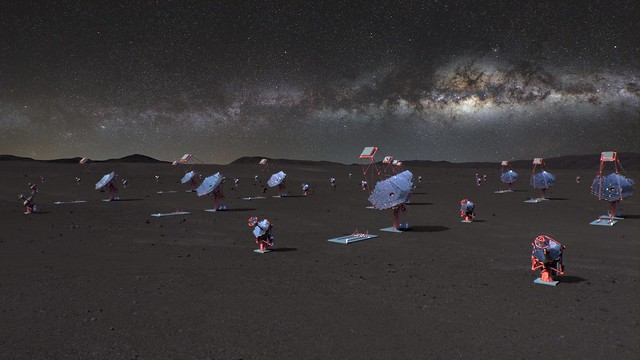
\includegraphics[height=0.18428\textwidth]{figures/telescopes/CTA.jpg}%

        \begin{itemize}
            \item We are moving from an age of \textbf{precision} cosmology to \textbf{accurate} cosmology.
            \item \textbf{Systematics} $\gtrsim$ \textbf{statistics}.
            \item Tools risk lagging behind hardware
        \end{itemize}

    \end{columns}
\end{frame}

\begin{frame}
    \frametitle{Interdisciplinarity}
    Combining data and disciplines will be the key to breakthroughs

    INSERT graphic of combinations of data for DESI

    INSERT graphic of combinations of data for Particle physics

    INSERT graphic of combinations of data for PTAs

    INSERT graphic of combinations of data for astronomy (e.g. AGN)

    Interdisciplinarity gives two-way interchange of ideas

    (Diversity comment)

    Take you through a tour of how my research programme is well placed to do this
\end{frame}

\begin{frame}
    \frametitle{\textit{Planck}: Inflation \& primordial power spectrum}

    Began PhD in initial conditions for inflation

    Joined Planck inflation team

    Performing model comparison fits 

    FlexKnots

    (could merge with next slide)
\end{frame}

\begin{frame}
    \frametitle{From \texttt{MultiNest} to \texttt{PolyChord}}
    Emphasise key theoretical skills that come from a background in theoretical ideas giving breakthroughs in theory of nested sampling

    then implementation in practice into software

    Enabling analyses that were not possible (axions)
\end{frame}

\begin{frame}
    \frametitle{Aside: theoretical work}

    Whilst I maintain an interest in the theoretical side of cosmology, the law of evolution shows inevitably there is higher impact (and likely higher interest) in the interdisciplinary work that I do

    cursory slide on:

    - quantum fields in curved spacetime

    - future conformal boundary/CPT

    - curved primordial power spectra equations

    - Poincare gauge theory

    danielle, will, sinah
\end{frame}

\begin{frame}
    \frametitle{Interdisciplinary work to date}

    List of all of the work I have done
    \begin{itemize}
        \item Exoplanets
        \item 21cm cosmology
        \item Radio Instrumentation
        \item Gravitational waves
        \item Industry
            \begin{itemize}
                \item Battery technology
                \item Finance
                \item Defence
                \item Protein folding
            \end{itemize}
        \item Particle physics
        \item Theory of machine learning
    \end{itemize}

    Highlight the ones I'm actually going to mention
\end{frame}

\begin{frame}
    \frametitle{Nested sampling: \texttt{PolyChord}, \texttt{anesthetic} \& beyond}
    Let's get the obvious one out of the way

    Lukas Hergt, David Yallup, Adam Ormondroyd

    presenting work on DiffusionNS -- nested sampling powerd by diffusion models
\end{frame}

\begin{frame}
    \frametitle{21cm cosmology}

    flexknots (ideas that came from Galaxies/Cosmo)

    maxsmooth (ideas that came from working in finance)

    margarine (ideas that came from CMB/ML)
\end{frame}

\begin{frame}
    \frametitle{REACH:}

    radiometry

    model fitting

    antenna design

    cutting edge machine learning methods
\end{frame}

\begin{frame}
    \frametitle{Gravitational waves}
    Alvin and Metha

    General usage within GW community
\end{frame}

\begin{frame}
    \frametitle{Exoplanets}
    Work with Didier

    Interest in Madhu's programme

    Other crosdisciplinary chemistry work 
\end{frame}

\begin{frame}
    \frametitle{GAMBIT}
    \framesubtitle{Interdisciplinary case studies}
    \begin{columns}
        \column{0.5\textwidth}
        \begin{itemize}
            \item GAMBIT is an interdisciplinary community and software framework.
            \item Like \texttt{CosmoMC}/\texttt{Cobaya}/\texttt{Bilby}, an organiser of data, likelihoods \& theory, including:
                \begin{itemize}
                    \item Collider data (e.g. LHC)
                    \item Direct detections (e.g. XENON1T)
                    \item Cosmology (MontePython)
                    \item Astrophysics (e.g. Bullet Cluster, Supernovae)
                    \item Pulsar timing
                    \item \ldots \& much more
                \end{itemize}
            \item \texttt{GravBit} and \texttt{LowEnergyBit} arising from GAMBIT@KICC workshop
        \end{itemize}
        \column{0.5\textwidth}
        
\includegraphics[height=0.423\textwidth]{figures/students/gambit.png}
        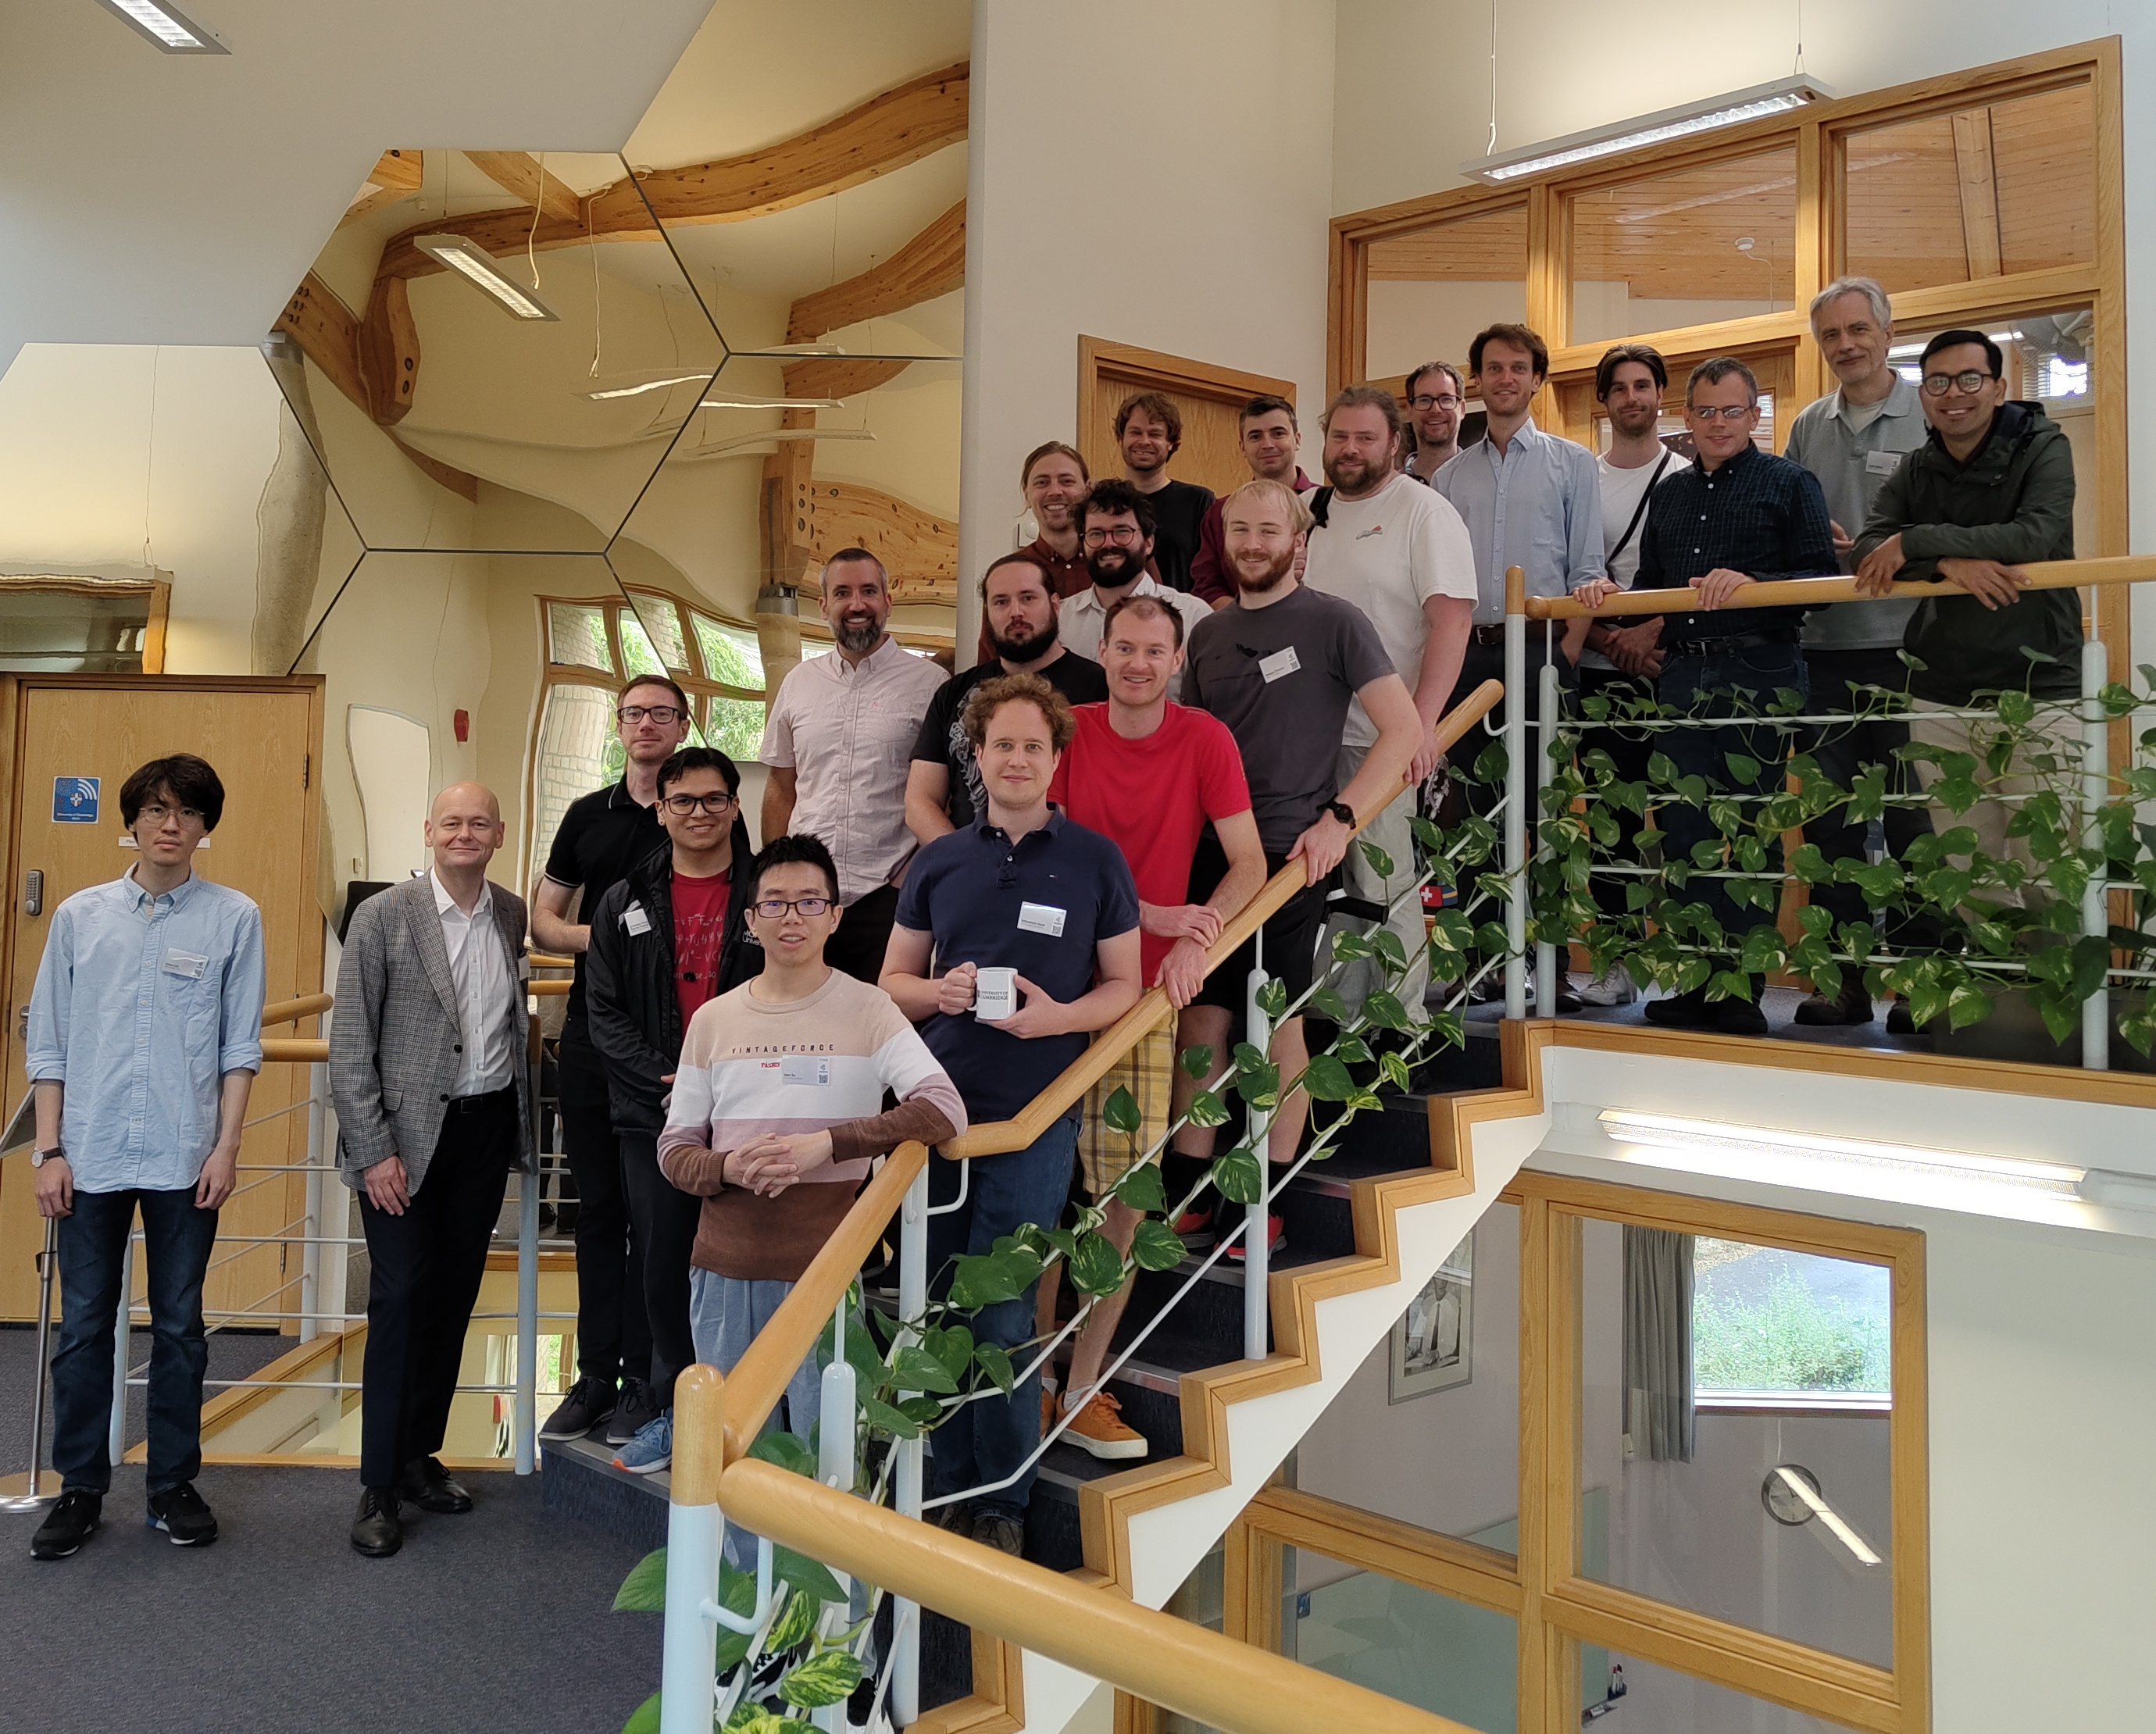
\includegraphics[height=0.423\textwidth]{figures/gambit_kicc.jpg}
        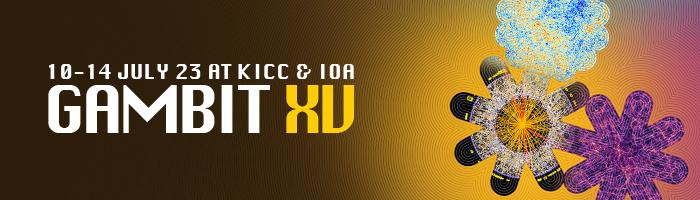
\includegraphics[width=\textwidth]{figures/gambit_meetingbanner.jpg}
    \end{columns}
\end{frame}

\begin{frame}
    \frametitle{GAMBIT: sub-GeV Dark matter constraints}
    \framesubtitle{Interdisciplinary case studies}
    \student{gambit}{Felix Kahlhoefer et al}{GAMBIT cosmo/DM working group}
    \begin{columns}
        \column{0.56\textwidth}
        \begin{itemize}
            \item Physical model of sub-GeV thermal dark matter with a dark photon mediator~$A$:
        \end{itemize}
        \vspace{-10pt}
        \begin{align*}
            \small
            \mathcal{L}_\text{int} =& -\frac{1}{2} m_{A'}^2 A'^\mu A'_\mu - \frac{1}{4} A'^{\mu\nu}A'_{\mu\nu} -\kappa e A'^\mu \sum_{f} q_f \overline{f} \gamma_\mu f \,,
            \normalsize
        \end{align*}
        \vspace{-15pt}
        \begin{itemize}
            \item Constrain using cosmological, astrophysical, accelerator \& direct detection data.
            \item Bayesian Model comparison of Fermion~$\psi$ vs scalar~$\Phi$ models (scalar preferred).
        \end{itemize}
        \vspace{-10pt}
        \begin{align*}
            \small
            \mathcal{L}_\psi  =& \bar{\psi}(i \slashed{\partial} - m_\text{DM}) \psi + g_\text{DM} A'^\mu \bar{\psi} \gamma_\mu \psi \,,\\
            \mathcal{L}_\Phi  =& |\partial_\mu \Phi|^2 - m_\text{DM}^2 |\Phi|^2 - g_\text{DM}^2 A'_\mu A'^\mu |\Phi|^2 \\ &+ i g_\text{DM} A'^\mu \left[\Phi^\ast (\partial_\mu \Phi) - (\partial_\mu \Phi^\ast) \Phi\right]\,,
            \normalsize
        \end{align*}
        \column{0.44\textwidth}
        \vspace{10pt}
        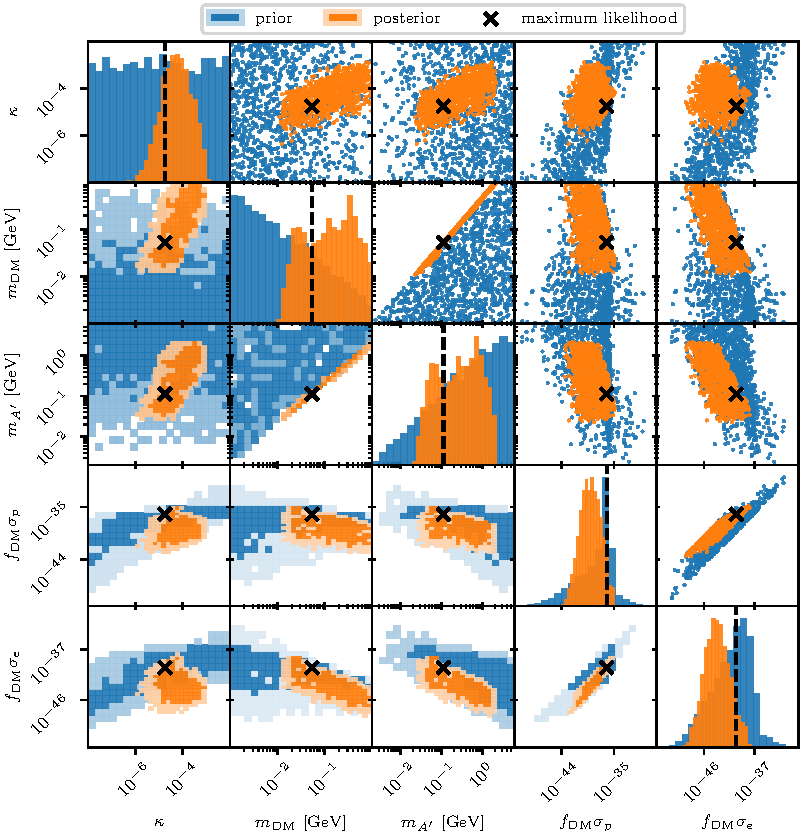
\includegraphics[width=\textwidth]{figures/Bayes_SubGeVDM_fermion_RDprior_allDM_asym_observables.pdf}
    \end{columns}
\end{frame}

\begin{frame}
    \frametitle{PolyChord Ltd}

\end{frame}

\begin{frame}
    \frametitle{DSTL: }
    \framesubtitle{Interdisciplinary case studies}
    Bayesian OODA loops
\end{frame}

\begin{frame}
    \frametitle{Tensions in cosmology}
    \begin{columns}
        \column{0.31\textwidth}
        \begin{block}{Hubble tension}
            <+Content+>
        \end{block}
        \column{0.31\textwidth}
        \begin{block}{Weak lensing tension}
            <+Content+>
        \end{block}
        \column{0.31\textwidth}
        \begin{block}{$w_0$/$\Omega_K$/$\nu$}
            <+Content+>
        \end{block}
    \end{columns}

    In order to disentangle systematics from statistics we need a new theory of data analysis

    Whilst we are all waiting for a new theory of the universe, we must also be prepared for the possibility that it at the largest scales $\Lambda$CDM really is the correcty phenomenological description.

    The redshift frontier of gravitational waves, 21cm SKA, and observations from the moon are what will really challenge our astronomical understanding.

\end{frame}

\begin{frame}
    \frametitle{The real tension in the room}

    \begin{columns}
        \column{0.31\textwidth}
        \begin{block}{Dark tension}
            <+Content+>
        \end{block}
        \column{0.31\textwidth}
        \begin{block}{Initial conditions}
            <+Content+>
        \end{block}
        \column{0.31\textwidth}
        \begin{block}{Quantum gravity}
            <+Content+>
        \end{block}
    \end{columns}
\end{frame}

\begin{frame}
    \frametitle{The future: simulation-based inference}

    This will be how everybody does it (evolutionary principles)

    We should ask ourselves why most people don't use LBI

    re-emphasise analytical work in the context of frontiers of data analysis

    PolySwyft \& LSBI
\end{frame}

\begin{frame}
    \frametitle{ERC grant: COSMOTENSION}
    \framesubtitle{Resolving cosmological tensions with diverse data, novel theories and Bayesian machine learning}

    \texttt{\tthref{willhandley.co.uk/ERC.pdf}}
\end{frame}

\begin{frame}
    \frametitle{Conclusions}
    \framesubtitle{\tthref{github.com/handley-lab}}
    %TODO
    Images of DiRAC, ERC, URF and PCLtd for resources at my disposal

    Interdisciplinarity of theory, observation and inference

    \tikz[overlay,remember picture]
    \node[anchor=north east] (A) at ($(current page.north east)+(0,0)$) {
        
\includegraphics[width=0.09\textheight]{figures/students/adam_ormondroyd.jpg}%
        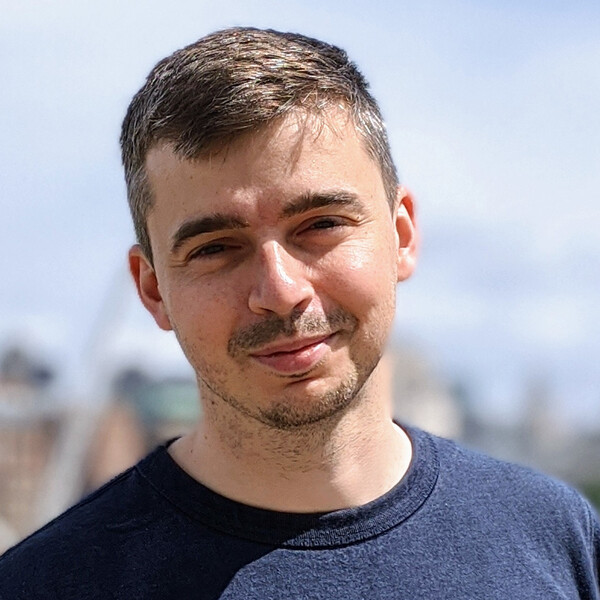
\includegraphics[width=0.09\textheight]{figures/students/david_yallup.jpg}%
        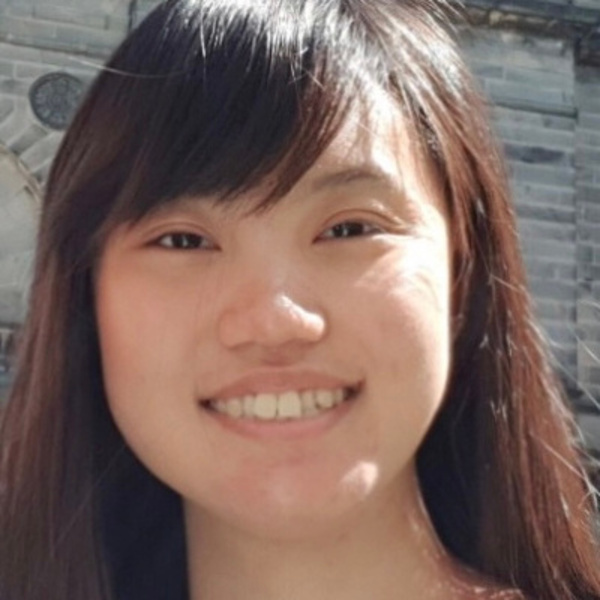
\includegraphics[width=0.09\textheight]{figures/students/dily_ong.jpg}%
        
\includegraphics[width=0.09\textheight]{figures/students/felicity_ibrahim.jpg}%
        
\includegraphics[width=0.09\textheight]{figures/students/george_carter.jpg}%
        
\includegraphics[width=0.09\textheight]{figures/students/harry_bevins.jpg}%
        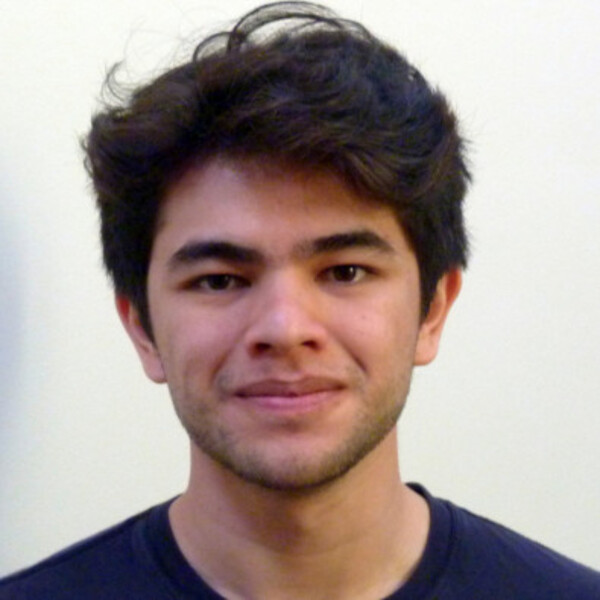
\includegraphics[width=0.09\textheight]{figures/students/ian_roque.jpg}%
        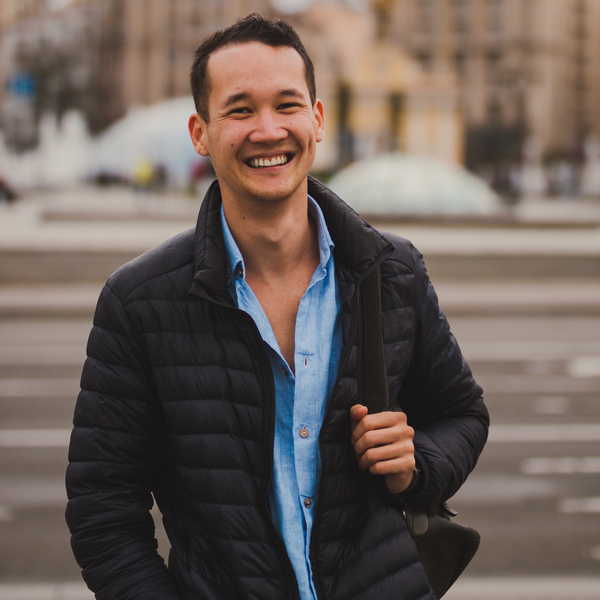
\includegraphics[width=0.09\textheight]{figures/students/kilian_scheutwinkel.jpg}%
        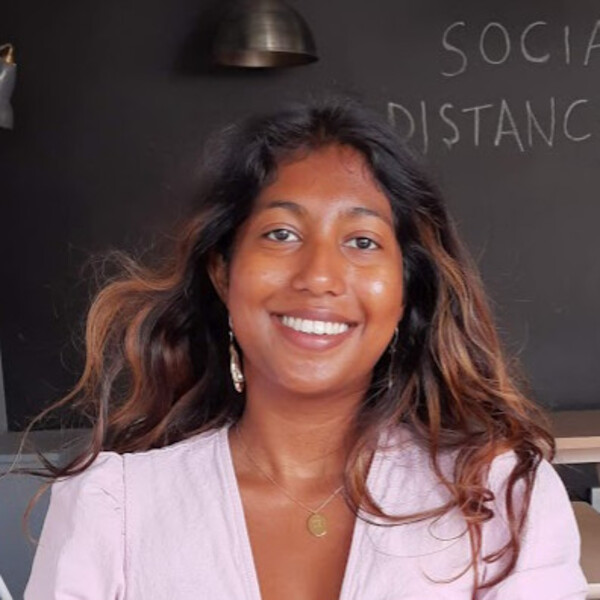
\includegraphics[width=0.09\textheight]{figures/students/metha_prathaban.jpg}%
        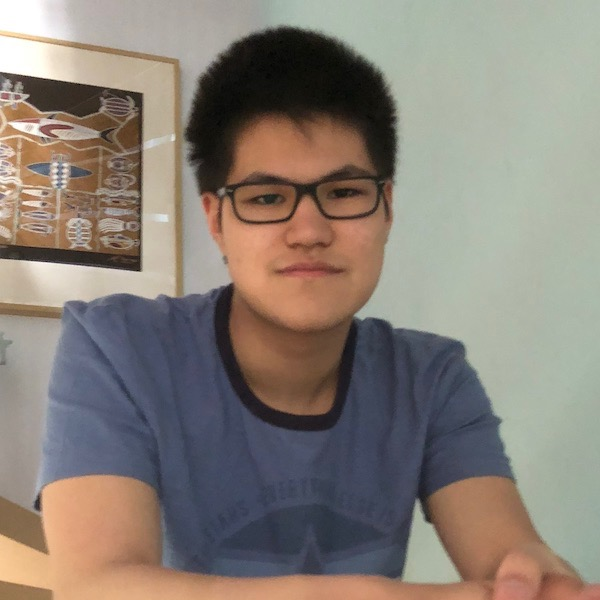
\includegraphics[width=0.09\textheight]{figures/students/namu_kroupa.jpg}%
        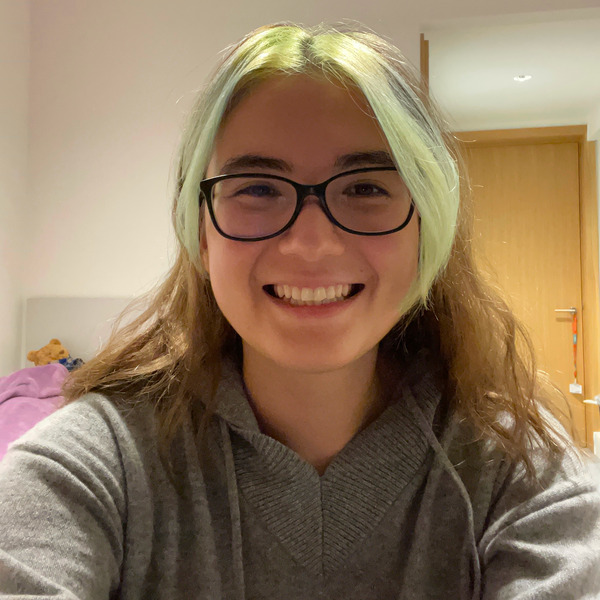
\includegraphics[width=0.09\textheight]{figures/students/sinah_legner.jpg}%
        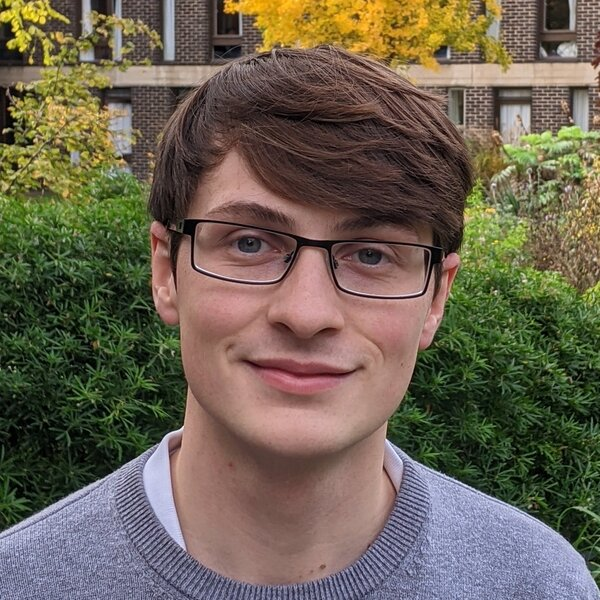
\includegraphics[width=0.09\textheight]{figures/students/thomas_gessey-jones.jpg}%
        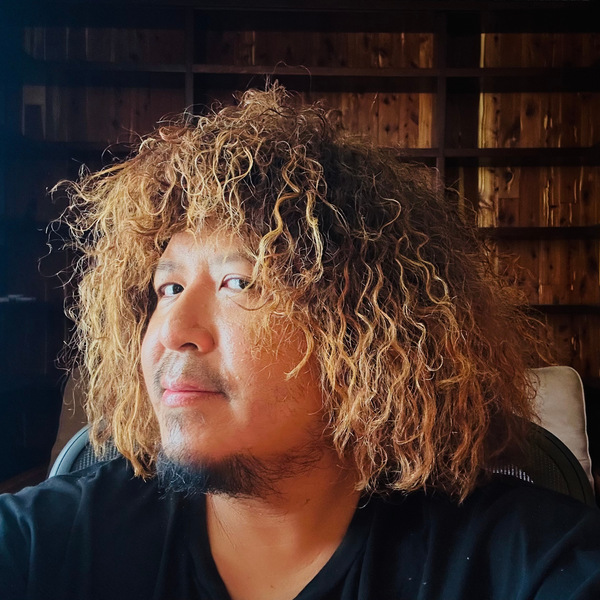
\includegraphics[width=0.09\textheight]{figures/students/tze_goh.jpg}%
        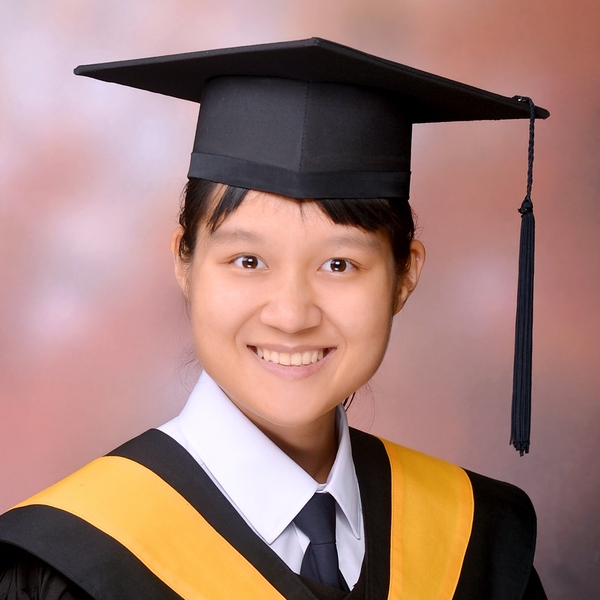
\includegraphics[width=0.09\textheight]{figures/students/wei-ning_deng.jpg}%
    };
\end{frame}


%\begin{frame}
%    \frametitle{unimpeded: PLA for the next generation}
%    \student{dily_ong}{Dily Ong}{PhD}
%    \begin{columns}
%        \column{0.5\textwidth}
%        \begin{itemize}
%            \item DiRAC 2020 RAC allocation of 30MCPUh
%            \item Main goal: Planck Legacy Archive equivalent
%            \item Parameter estimation $\to$ Model comparison
%            \item MCMC $\to$ Nested sampling
%            \item Planck $\to$ $\{\text{Planck}, \text{DESY1}, \text{BAO}, \ldots \}$
%            \item Pairwise combinations
%            \item Suite of tools for processing these 
%                \begin{itemize}
%                    \item \texttt{anesthetic} $2.0$
%                    \item \texttt{unimpeded} $1.0$
%                    \item \texttt{zenodo} archive
%                    \item \texttt{margarine}
%                \end{itemize}
%            \item MCMC chains also available.
%            \item Library of bijectors emulators for fast re-use
%        \end{itemize}
%        \column{0.5\textwidth}
%        
\includegraphics[width=\textwidth]{logos/dirac.png}
%        \includegraphics[width=0.5\textwidth,page=21]{figures/himmelblau.pdf}%
%        \includegraphics[width=0.5\textwidth,page=15]{figures/himmelblau.pdf}
%    \end{columns}
%\end{frame}




%\begin{frame}
%    \frametitle{Other frontiers}
%    Copilot
%
%    ChatGPT
%
%    LLMs/translation between disciplines
%    
%\end{frame}

\end{document}
